\chapter{Available Functionality and How to Use It}
\label{ch:modules}
% ##################################################################################################################

\hfill \textbf{Authors:} Andreas Horni, Kai Nagel

\begin{center} 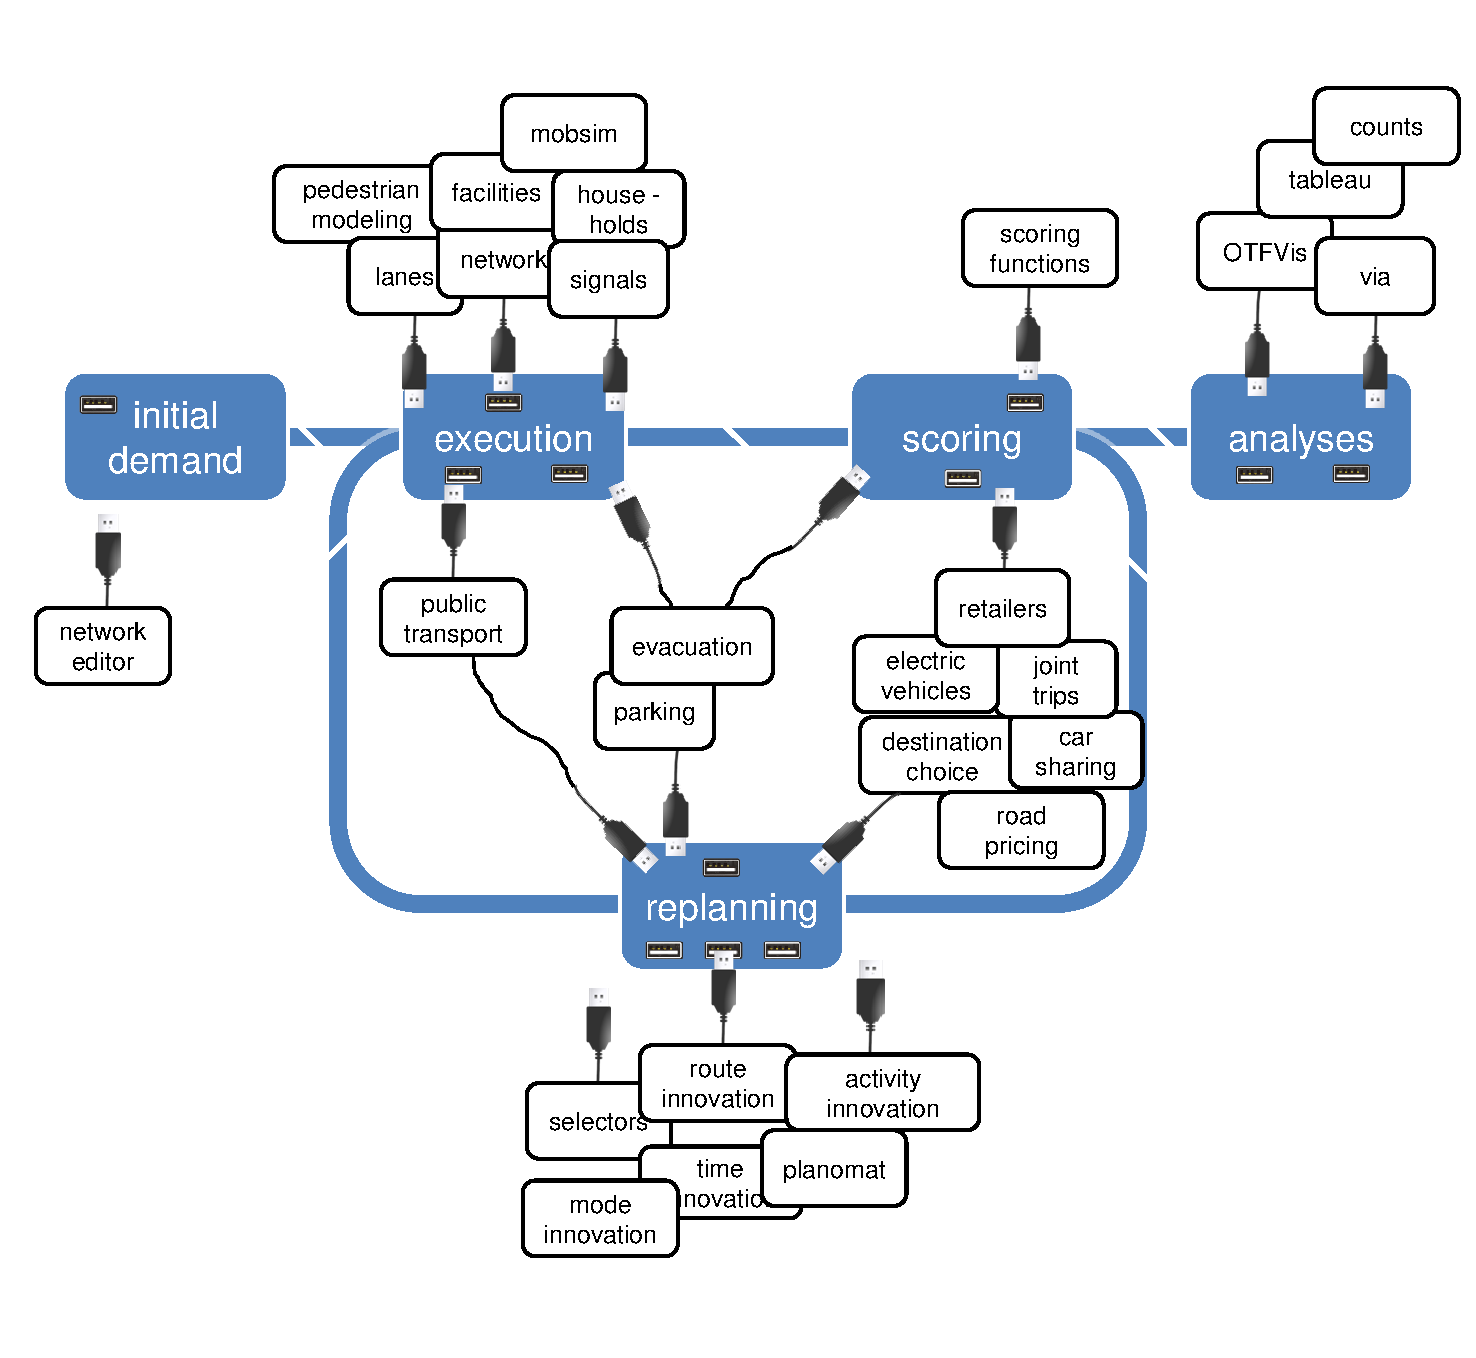
\includegraphics[width=0.5\textwidth, angle=0]{extending/figures/modules.pdf} \end{center}

%% \kaitodo[inline]{read chapter/section}

%% \atend{re-read modules.tex just before going to print}

%%%%%%%%%%%%%%%%%%%%%%%%%%%%%%%%%%%%%%%%%%%%
%%%%%%%%%%%%%%%%%%%%%%%%%%%%%%%%%%%%%%%%%%%%
%\kai{need to clarify the factory concept somewhere (in the future probably just PopulationUtils.createActivity(...)).}
%
%\ah{Section~\ref{sec:extending-initial-demand}}
%
%\ah{added ``events'' module under ``Global Modules and Global Aspects''}

%%%%%%%%%%%%%%%%%%%%%%%%%%%%%%%%%%%%%%%%%%%%
%%%%%%%%%%%%%%%%%%%%%%%%%%%%%%%%%%%%%%%%%%%%

% ##################################################################################################################
In this chapter you will learn about possibilities to extend and customize \gls{matsim} through provided functionality. 
In Chapter~\ref{ch:extensionpoints}, you will see how you can hook your own extensions into \gls{matsim}.

%%\kai{Frage mich im Moment, ob wir diejenigen ``Module'', die man per config aufrufen kann, nicht doch lieber bereits unter ``using'' beschreiben sollten.  Aber vielleicht ist das inzwischen fast egal, und wir sollten lieber Standard-MATSim komplett separat von jeder Art Variation halten.  ???}
%\ah{see Chapter~\ref{ch:configuring}}

% ##################################################################################################################
\section{MATSim Modularity}
\label{sec:matsim-modularity}

%% \kai{Andreas, haben wir noch eine Chance, diese Ungleichheiten in der Nomenklatur geradezuziehen?  
%% %contrib vs extension \url{https://matsim.atlassian.net/browse/MATSIM-323};  
%% PlanStrategy vs StrategyModule; ... } \kai{M.E.\ gelöst mit der Umbenennung in Thibaut's neuer Syntax.}

% ====================================================================================================
MATSim follows a modular concept, but
a ``module'' is not a very specific term;\footnote{
According to the Merriam-Webster (\url{http://www.merriam-webster.com}), a module is
%
``one of a set of parts that can be connected or combined to build or complete something'' 
%
or more specifically
%
``a part of a computer or computer program that does a particular job''. 
%
} thus, modules can exist at many levels in a software framework.
Also in MATSim, a range of different functionality types, such as
config functions,
replanning components,
contributions,
or even 
external tools,\footnote{Standalone tools referencing \gls{matsim} as a library, such as the network editor, or the visualizer \gls{via}.}
are sometimes described as modules. 
Metaphorically speaking, module can thus be seen as the greatest common divisor (gcd) of different functionality provided in \gls{matsim}.
Much more important is understanding the different levels of access stemming from the generally modular architecture.

% ====================================================================================================
\subsection{Levels of Access}
\label{sec:levels-of-access}
\gls{matsim} currently provides five levels of access: 
\begin{enumerate}\styleEnumerate
\item using the \gls{matsim} core only, 
\item using the \gls{matsim} main distribution, 
\item using \gls{matsim} main distribution, \glspl{contribution} and possibly extensions,
\item writing ``scripts in \gls{java}'' and finally 
\item  writing your own \glspl{extension}.
\end{enumerate}

% --------------------------------------------------------------------------------------
\subsubsection{Using the Core Only}
\label{sec:using-core-only}

%% \kai{würde gerne, hier und im folgenden, url links auf sourceforge gerne vermeiden ... wir haben da keine Kontrolle drüber, ob die sich ändern.  M.E.\ lieber auf so etwas wie matsim.org/downloads verweisen.}

To use only the core, one needs to do the following (see Section~\ref{sec:runningmatsim}):
\begin{itemize}\styleItemize
\item Download a \gls{matsim} release or a nightly build, by following the respective links at %% \url{http://sourceforge.net/projects/matsim/files/} or a nightly build \url{http://matsim.org/downloads/nightly} % \kai{url?}.
\url{http://matsim.org/downloads}.
\item Obtain a network file and an initial plans file.  Small versions can be typed by hand; larger versions should be generated automatically by some computational method.
\item Write or edit a \gls{configfile}.
\item Click on the \gls{matsim} jar file\footnote{This has worked since winter 2014/15 and should be in the 0.8.x~release.} and follow the instructions. 
\end{itemize}
We think that the \gls{matsim} core is already quite powerful; for example, synthetic persons already follow full daily plans with a full daily scoring function; thus, opening times for activity types, departure time choice and schedule delay can be investigated. 
% Also, schedule-based public transit assignment is contained in the core. \ah{not according to current def of core}

% --------------------------------------------------------------------------------------
\subsubsection{Using MATSim Main Distribution}
\label{sec:using-main-distro}
The \glspl{extension} in the \gls{matsim} main distribution are, by design, very close to the \gls{matsim} core, thus requiring even less configuration than for \glspl{contribution}, as shown below. Often, providing additional files together with a respective \gls{configfile} entry is sufficient to use them; required steps are described below, case by case. Extensions contained in the main distribution are listed in a separate section at \url{http://matsim.org/extensions}.

% --------------------------------------------------------------------------------------
\subsubsection{Using One or More Contribs or Other Extensions}
\label{sec:using-contribs}
%\kai{Das wären jetzt eigentlich extensions; ``contribs'' sind diejenigen extensions, die sich gleichzeitig im matsim repository befinden.  Oder?}
%\ah{Nein, gemäss momentaner Buch-Definition liegen contribs unter ``contribs'', Module, welche über config, pop, network hinausgehen, aber im Core (was immer das nun genau ist) liegen, haben im Moment keinen Namen.}
%\ah{geklärt}
%
\Glspl{contribution} are in a separate part of the repository, separate from the \gls{matsim} main distribution.  
The documentation is not yet fully organized; information about \glspl{contribution} and other extensions can be found at 
%\url{http://matsim.org/javadoc} or 
\url{http://matsim.org/extensions}. 
For the \glspl{contribution}, there are also release versions and nightly builds, which can be found by following the links at %\url{http://sourceforge.net/projects/matsim/files/} 
%\url{http://matsim.org/files/builds/}. % \kai{check} \ah{gibt es beides am gleichen Ort wie MATSim} \kai{url?}.
\url{http://matsim.org/downloads}.

In general, \glspl{contribution} should provide main methods for usage.  
We may eventually provide clickable jar files here as well, but, for the time being, contributions need to be bundled with core \gls{matsim} (and potentially other \glspl{contribution}). 
As shown at \url{http://www.matsim.org/docs/extensions}, the syntax---roughly---is
\begin{lstlisting}
java -Xmx2000m -cp MATSim.jar:contrib/contrib.jar org.matsim.contrib.run.RunXxx config.xml  
\end{lstlisting}
%% \kai{Maybe better point to electronic docu?} \ah{command ist unter url oben gegeben}
where
\begin{itemize}\styleItemize
\item \lstinline$-Xmx2000m$ increases the \gls{java} heap space, so that most \gls{matsim} runs fit in
\item \lstinline$MATSim.jar$ needs to be replaced by a relative or absolute path to the \gls{matsim} jar to be used
\item \lstinline$contrib/contrib.jar$ needs to be replaced by a relative or absolute path to the \gls{contribution} jar to be used
\item \lstinline$org.matsim.contrib.run.RunXxx$ needs to be replaced by the full \gls{java} class name containing the desired main method (given by the \gls{contribution} documentation)
\item \lstinline$config.xml$ needs to be replaced by a relative or absolute path to a \gls{configfile}, which may contain additional sections specific to the \gls{contribution}.
\end{itemize}

It is possible to combine several \glspl{contribution} in this way, provided someone has made a corresponding main method available.  This can, in principle, be done relatively quickly, so those wishing to run studies with combinations of existing \glspl{contribution}, but without programming skills, can ask someone with those skills and with access to the repository for help.

% --------------------------------------------------------------------------------------
\subsubsection{Writing \enquote{Scripts in Java}}
\label{sec:writing-scripts-java}
The \glspl{contribution} are written so that they can be plugged into \gls{matsim} via extension points (see Chapter~\ref{ch:extensionpoints}). 
If a specific combination or configuration of modules is not (yet) available, one can write it. The syntax roughly is:
\begin{lstlisting}
... main( ... ) {
    // construct the config object:
    Config config = ConfigUtils.xxx(...) ;
    config.xxx().setYyy(...) ;
    ...

    // load and adapt the scenario object:
    Scenario scenario = ScenarioUtils.loadScenario( config ) ;
    scenario.getXxx().doYyy(...) ; // (*)
    ...

    // load and adapt the controler object:
    Controler controler = new Controler( scenario ) ;
    controler.doZzz(...) ; // (**)
    ...

    // run the iterations:
    controler.run() ;
}
\end{lstlisting}
Extension points, especially at \lstinline{(*)} and \lstinline{(**)}, are described in more detail in Chapter~\ref{ch:extensionpoints}.

% --------------------------------------------------------------------------------------
\subsubsection{Writing Your Own Extensions}
\label{sec:writing-your-own-extensions}
If the existing \glspl{extension} are not sufficient to plug your own study together, the next option is to write your own \gls{extension}. 
Again, when writing an \gls{extension}, one should use the extension points described in Chapter~\ref{ch:extensionpoints}, since this is the only way an \gls{extension} can later become a \gls{contribution}. 

%\pararaph{Config Parameters:}
%\gls{matsim} provides the possibility that the parameters of arbitrary and also external modules are added to the configuration file. 
%In the respective module, the parameters can be accessed in two ways. The suggested way is extended the \lstinline|Config| object to include an external config group as follows.
%%
%\begin{lstlisting}
%MyExternalConfigGroup myConfig = ConfigUtils.addOrGetModule(controler.getConfig(), MyExternalConfigGroup.GROUP_NAME, MyExternalConfigGroup.class);
%\end{lstlisting}
%%
%Parameters are then available by the getter methods of \lstinline|MyExternalConfigGroup|. A second way, is using the following command of the \lstinline|Config| class.
%\begin{lstlisting}
%public final String findParam(final String moduleName, final String paramName)| 
%\end{lstlisting}
%Note, that here, the user's input is not checked while reading in the \gls{configfile} but much later, possibly in the external module.
%
%\kai{MZ, wollen wir dieses findParam eigentlich noch ``advertisen''?  Bisher ist es immer darauf hinausgelaufen, dass ich das irgendwann durch eine "typisierte" config group ersetzt habe.  M.E.\ könnte man zukünftig auch gleich mit einer typisierten config group anfangen.  Oder?}
%\ah{Hab mal beides hingeschrieben. Michael: Ist eines von beidem empfohlen? ;)}
%\ah{moved this to Section~\ref{sec:config}}

%\kai{here is a difference between an extension and a contrib :--)}

%% \paragraph{If none of this is enough}
%% Clearly, it is always possible to download some version of \gls{matsim}, remove all the \lstinline{final} 

% ====================================================================================================
\subsection{The Ideas Behind this Setup}
The setup, as described above, arose from the observation that an-ever growing monolithic \gls{matsim} would eventually overwhelm the \gls{matsim} team and its core developers group. 
Therefore, a set-up was sought allowing them to concentrate on central infrastructure, while specific functionality like road pricing, \gls{multimodal} simulations, signals, additional choice dimensions, or analysis modules could be written and contributed by the community. 
Clearly, a plug-in architecture had to be the solution, but it took (and still takes) time and effort to make the extension points sufficiently capable and robust.  

At the same time, \gls{matsim} is a research platform; research investigates innovative questions, which often means that the questions were not foreseen when the code was designed. 
Quite often, scripting languages are the solution to such problems; 
for example, python is allowed in \gls{qgis},\footnote{\url{http://docs.qgis.org/testing/en/docs/pyqgis_developer_cookbook/}} %\ah{keep url here because of python}
\gls{visum},\footnote{\citep{VISUM_manualNewFeatures_2011}} %\ah{keep url here}
\gls{emme}, or 
\gls{sumo} (via the TraCI interface)\footnote{\url{http://sumo.dlr.de/wiki/TraCI}} % \ah{keep url here because of traci}
for plug-ins.
%\ah{have to put urls in bib}
%\kai{Wir könnten generell darüber nachdenken, bei Abkürzungen die Referenzen im acronyms.tex zu geben.}
%\ah{made it a todo item}
\gls{scala} 
was discussed for \gls{matsim}, but ultimately, it was decided to just use \gls{java} itself as the scripting language, 
with the advantage that users  between development and \gls{matsim} application do not need to learn two languages. 
In addition, the \gls{tu} Berlin team can continue to teach \gls{java} both as an entry point to \gls{matsim} and as a general professional skill.

% ====================================================================================================
%\subsection{MATSim Modules}

%\ah{Mittlerweile frage ich mich, ob wir nicht einfach zusammenfassend sagen sollten, dass es verschiedene Ausprägungen von Modulen gibt und Untenstehendes auf 2-3 Sätze zusammengepresst werden sollte. Eine weitere Klassifikationsmöglichkeit brauchen wir nicht, vor allem nicht wenn es nur eine Klasse gibt ;)
%Mit deinem OK versuche ich das mal.}
%
%That is, ``module'' is not a very specific term, and in consequence modules exist in \gls{matsim} at many levels. 
%Metaphorically speaking, the term module can thus be seen as the greatest common divisor (gcd) of different functionality provided in \gls{matsim}.
%%% , so to say, a module is the \lstinline|AbstractClass| of \gls{matsim} functionality. 
%%
%% Eine abstrakte Klasse im Java-Sinne ist ein nicht einfaches Software design Konzept; das würde ich hier nur ungern nennen. kai, jan'15
%As \gls{matsim} is 
%highly modular, it nevertheless makes sense to think of functionality wrapped by a module. In the following are some important examples.

%% The basic concept to extend MATSim is the usage of modules. But, please be aware that when it comes to configuring MATSim the term ``module'' is very extensively used such that a clear definition of what is a module and what is not is not available to date. This consequence of organic grows be corrected on the long run, for now, we try to just sort out the different meanings of the word module

%% \kai{Ich bilde mir ein, dass wir das im Kopf schon etwas klarer haben, als es historisch noch aussieht, und würde gerne versuchen, das hier zu kommunizieren.  Ich habe in der Einleitung zu Kap.~\ref{ch:extensionpoints} etwas geschrieben, was man vielleicht inhaltlich auch hier verwenden kann ...}

%% Following different components are called modules.

%% \paragraph{Components in \lstinline|org.matsim|:} % --------------
% ...........................................................................
%\paragraph{Config Modules:} The config \gls{xml} file uses a syntax of the type
%\begin{xml}
%<module name="aModule">
    %<param name="aParameterForAModule0" value="someValueX" />
    %<param name="aParameterForAModule1" value="someValueY" />
%</module>
%\end{xml}
%The config modules loosely correspond to components providing distinct functionality. 
%
%%% residing in the \lstinline|org.matsim| package.  
%
%%% Habe das mal auskommentiert.  Ist erstens eine Null-Aussage (alles ist unterhalb von org.matsim, auch die contribs), und zweitens ist es wenigstens im Java-Sinne keine package (oder genauer: Gerade in dieser package ist nichts drin). kai, dec'14
%
%{\footnotesize
%
%\kai{Andreas, habe obige Argumentation mal umgedreht.  Du bist von der code Struktur zum config file gegangen.  Ich gehe jetzt vom config file aus, und erwähne den code nur beiläufig.  Grund: Die beiden hängen tatsächlich nicht besonders stark zusammen.  Insbesondere passen wir die config, wg. Rückwärts-Kompatibilität, praktisch nie an strukturelle Änderungen im Code an.  (Abgesehen davon ist die config Struktur gar nicht so schlecht; problematisch finde ich teilweise eher die Benennungen.  Ein Favorit: ``planCalcScore'' (ohne s hinter plan) vs ''plansCalcRoute'' (mit s hinter plan). Oder?)}
%
%}
% ...........................................................................
%\paragraph{Replanning Modules:} Package \lstinline|org.matsim.core.replanning.modules| provides replanning functionality that can also be plugged into \gls{matsim}. 
%
%%% A slightly different meaning of modules, which is only relevant for the MATSim developer and API-user, is as follows. In the package package \lstinline|org.matsim.core.replanning.modules| replanning functionality is provided in classes that are derived from \lstinline|AbstractMultithreadedModule|.
%
%\kai{Dies ist mein zweiter Favorit.  ``(strategy)module'' in der config, aber ``PlanStrategy'' im code, die dann wieder ``PlanStrategyModule''s akzeptiert.  Schaffen wir es, dies aus Anlass des Buches zu ändern?  Siehe \url{https://matsim.atlassian.net/browse/MATSIM-306}.  Bitte äußere Dich dort (kann ja kurz sein).}
%\ah{Hab mal gevoted. Viel Zusätzliches zu sagen gibt es ja nicht ;)}
%%
%\kai{Lasse das bis zur Klärung dieser Frage mal offen.}
%%
%\kai{Das ist m.E.\ (für config v2) nun beseitigt.}

% ...........................................................................
%\paragraph{Contributions:} \Glspl{contribution} are modules residing in the \lstinline|org.matsim.contrib| package.
%
%\kai{Von mir aus können wir das durchgängig ``contribs'' oder ``contributions'' oder ``extensions'' nennen.  Leider hat Marcel für die package einen anderen Namen (contrib) gewählt als für die Doku (extensions).  Aber ``module'' muss nicht sein.}
%%
%\ah{Könnten wir sie trotzdem als Modul bezeichnen (einfach mit weniger negativem Unterton)? Die Story wird sonst sehr unübersichtlich (auch Kapitel "`Your Own Modules/Extensions...). Die anderen Probleme mit dem inflationären Gebrauch des Begriff bleiben ja.}
%%
%\kai{Verstehe das Argument.  Andererseits wird es auch nicht einfacher, wenn wir die Sprache nicht konsistent halten.  Hm.}
%
%\ah{Aus meiner Sicht ist "Modul" einfach der ggT oder die AbstractClass der verschiedenen Arten von ... Funktionalitäten (und somit eigentlich nutzlos?). Jedenfalls würde ich sie hier doch als Module bezeichnen, da sie sonst auch aus diesem Kapitel raus müssten.}
%
%\ah{Habe das oben mal (noch etwas blumig) angepasst.}

% ...........................................................................
%\paragraph{External Functionality:} % --------------
%Also external components plugged in and replacing a \gls{matsim} module, such as a \gls{mobsim}, can be interpreted as modules.

% ...........................................................................
%\paragraph{Standalone Tools:} % --------------
%Also the standalone tools referencing \gls{matsim} as a library, such as the network editor, or the visualizer \gls{via}, can be seen as modules.
%are termed modules in current practice.


% ===================================================================================
%\subsection{Current Problems With Modules}
%
%\kai{Habe diesen ganzen Abschnitt mal probehalber auskommentiert.  Module können auf vielen Ebenen auftreten, dass sie das tun, ist kein Fehler.  Manche der Aspekte können wir immer noch in den spezifischen Kapiteln beschreiben (es gibt tatsächlich einen Grund, warum es die ganzen unterschiedlichen mode innovation modules gibt); manche können wir vielleicht noch vor Fertigstellung des Buches im Code aufräumen.}

%% The majority of the replanning modules have their own section in the configuration file, but some do not, such as the \lstinline|TripsToLegsModule|. 
%% \kai{Aber warum ist das ein Problem?  Die sind halt nicht weiter konfigurierbar.}
%% %
%% In that package---called modules---there are furthermore, the factories for the plan selectors. For the selectors and their factories, it is unclear if they are modules.
%% \kai{factories sind keine modules, sondern extension points, um module zu erzeugen und in den code zu stöpseln.  Selectors selber sind PlanStrategies und insofern modulare Bestandteile.}

%% To make things worse, there are cases where module names in the configuration file are not (yet) consistent with the naming in the code. Examples are ``\lstinline|strategy|'' in the configuration file and ``\lstinline|StrategyManager|'' in the code, or ``strategy module'' in the config file and ``\lstinline|PlanStrategy|'' in the code \ah{Nochmals nachsehen!}. Furthermore, modules are atomic. There is, for example, a module called ``\lstinline|ChangeSingleLegMod|'', a module ``\lstinline|ChangeLegMode|'' and a module ``\lstinline|SubtourModeChoic|'' instead of one single module called ``\lstinline|ModeChoice|''. This, on the one hand, has historical reasons; the three modules were developed temporally separated. On the other hand, the parameter set for a module is only minimal and unambiguous if provided for atomic modules as different parameters are required for the three modules.

%\ah{Habs noch ganz auskommentiert.}

% ##################################################################################################################
\section{An Overview of Existing MATSim Functionality}
Figure~\ref{fig:matsimmodules} shows where common \gls{matsim} modules are coupled with the \gls{matsim} loop. Some modules have a single connection point (shown around the loop, connected to the respective loop element), while others have multiple connection points (shown in the middle of the circle) and yet others work on a global range (shown on the left upper and lower corners).

%% Some modules were already presented in Chapter~\ref{ch:configuring}, while here it is shown how functionality can be extended further, using the \gls{configfile}, population and a network only. 
%(Can't say what the above sentence is supposed to mean. Maybe it got garbled.  At any rate, ch:configuring used config, pop, net only; here is about using more than that. kai, dec'15)
The technical details for module usage, in particular the parameter 
sets, are described at \matsimorg, especially \javadoc\ and \extensions.
%% in \citep[][]{MATSim_Userguide_2015} \todokai{rm usrguide} and in the \gls{javadoc}.

%% For the presentation of the available functionality, we chose to not use a single section per module but to group them according to common transport planning categories, in the example above this would be ``mode choice'' instead of the atomic categories, where we use terms ``functionality'' for the larger categories and ``module'' for the atomic components. %\kai{adapt table structure to revised chapter structure} \ah{erledigt}
%
% habe das mal auskommentiert; irgendwie ist es jetzt m.E. anders. kai, jul'15

%Due to 
As a result of the distributed and project- and dissertation-driven \gls{matsim} contribution process (see Chapter~\ref{ch:developmentprocess}), modules are often implemented for a specific practical purpose, leading to limitations of the respective module. For example, modules might only work for a specific mode, or for a defined calling order.  Normally, additional effort is needed to generalize the module;
% toward its embedding in the complete framework, 
in consequence, the combination of a specific module with other functionality is often a non-straight-forward task. This means that a user 
%is in charge of 
will have to systematically test any specific combination of modules before productively applying it.
%
\createfigure%
{MATSim functionality}%
{MATSim functionality}%
{\label{fig:matsimmodules}}%
{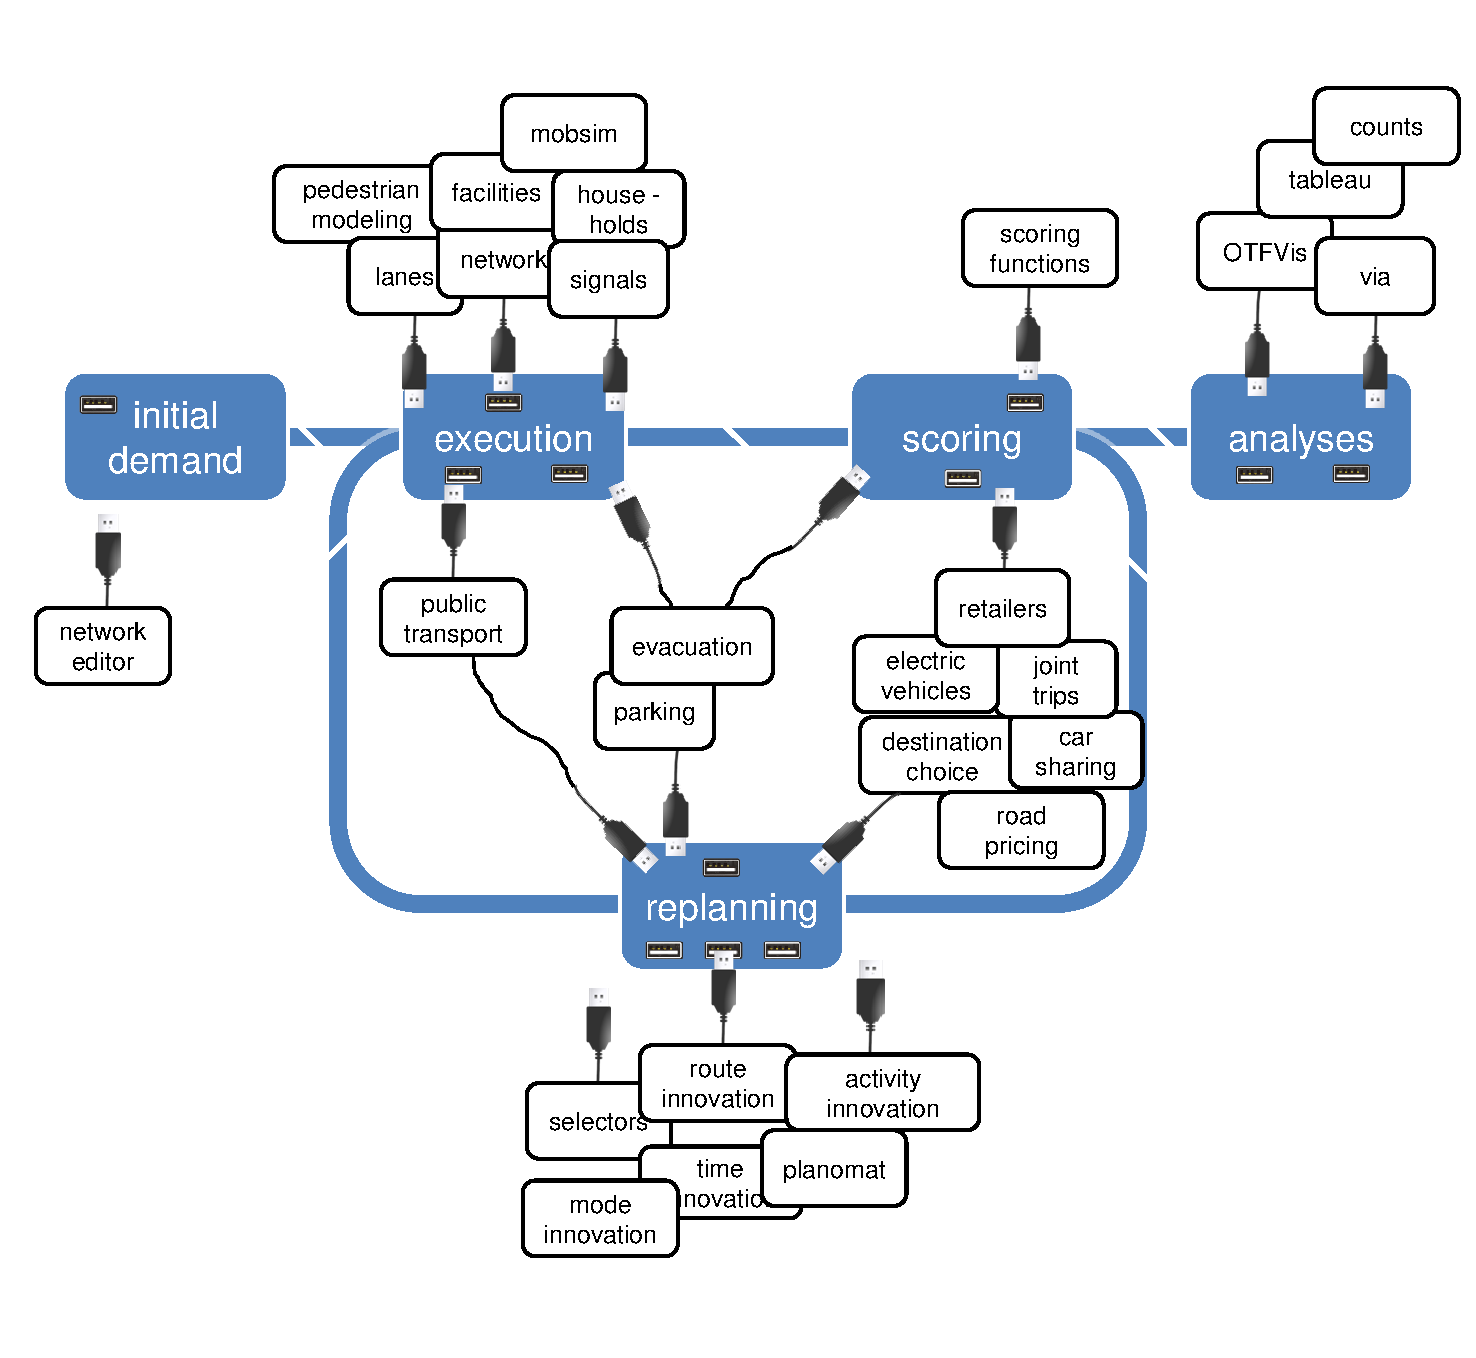
\includegraphics[width=0.99\textwidth, angle=0]{extending/figures/modules.pdf}}%
{}
The description of the modules in this, and the following chapters, is based on the categorization shown in Table~\ref{tab:modules}.
%
%\kai{TODO: macros for section names to re-use for table entries}
%\ah{Mache das später. Denke die jetzige Korrektur hält eine Weile}

\begin{center}
\begin{longtable}{|l|l|}
\caption{MATSim functionality overview}
\label{tab:modules} 
%\hline
%\textbf{Module} & \textbf{Type} &  \textbf{Described in} \\
%\hline
\endfirsthead
\hline
\multicolumn{2}{c}%
{\tablename\ \thetable\ -- \textit{Continued from previous page}} \\
\hline
%\textbf{Module} & \textbf{Type} &  \textbf{Described in} \\
%\hline
\endhead
\hline 
\multicolumn{2}{r}{\textit{Continued on next page}} \\
\endfoot
\hline
\endlastfoot
	\hline
	\textbf{MATSim Data Containers} & Section~\ref{sec:using-data-containers} and \ref{sec:extending-data-containers} \\
	\hline
	%% Scenario & Core & Section~\ref{sec:extending-scenario} \\
% gibt es nicht mehr. kai, jul'15
	Network  & Section~\ref{sec:using-network} and \ref{sec:extending-network} \\
	Population & Section~\ref{sec:using-population} and \ref{sec:extending-population} \\
	Counts  & Section~\ref{sec:extending-counts} \\
	Facilities & Section~\ref{sec:extending-facilities} \\
	Households & Section~\ref{sec:extending-households} \\
	Vehicles & Section~\ref{sec:extending-vehicles} \\
	Scenario & Section~\ref{sec:extending-scenario} \\
	\hline
	\textbf{Global Modules and Global Aspects} & Section~\ref{sec:using-globalmodules} \\ %and \ref{sec:extending-globalmodules} \\
	\hline
	Controler & Section~\ref{sec:using-controler} \\ %and \ref{sec:extending-controler} \\
	Events & Section~\ref{sec:using-events} \\
	Parallel Computing & Section~\ref{sec:using-paralleleventhandling} \\
	Global & Section~\ref{sec:using-global} \\
	\hline
	\textbf{Mobsims} & Section~\ref{sec:using-mobsims} and \ref{sec:extending-qsim} \\
	\hline
	QSim & Section~\ref{sec:using-qsim} and \ref{sec:extending-qsim} \\
	JDEQSim & Section~\ref{sec:using-jdeqsim} \\
	\hline
	\textbf{Scoring} & Section~\ref{sec:using-scoring} \\
	\hline
	\textbf{Strategy Modules} & Section~\ref{sec:strategymodules} \\
	\hline
	Time Innovation & Section~\ref{sec:timechoice} \\
	Route Innovation & Section~\ref{sec:routechoice} \\
	Mode Innovation & Section~\ref{sec:modechoice} \\
	Selectors & Section~\ref{sec:selectors} \\
	Destination Innovation & Chapter~\ref{ch:destinationchoice} \\
	\hline
	\textbf{Observational Modules} & Section~\ref{sec:observational} \\
	\hline
	Travel Time Calculator & Section~\ref{sec:ttc} \\
	Link Stats & Section~\ref{sec:linkStats} \\
	Analysis & Section~\ref{sec:contrib-analysis} \\
	Emissions & Chapter~\ref{ch:emissions} \\
	Accessibility & Chapter~\ref{ch:accessibility} \\
	\hline
	\textbf{Further Modules} &\\
	\hline
	Within-day Replanning & Chapter~\ref{ch:withinday} \\
	Public Transport & Chapter~\ref{ch:pt} \\
	Multi-Modal Contribution & Chapter~\ref{ch:multimodalsim} \\ % \ah{GTFS2TransitSchedule steckt da drin}
	Freight Traffic & Chapter~\ref{ch:freight} \\
	Car Sharing & Chapter~\ref{ch:carsharing} \\
	Joint Trips and Social Networks & Chapter~\ref{ch:jointtrips} \\
	Dynamic Transport Systems & Chapter~\ref{ch:dts} \\
	Parking & Chapter~\ref{ch:parking} \\
	Electric Vehicles & Chapter~\ref{ch:elvehicles} \\
	%Air and Rail Transport & (see PT) & Chapter~\ref{ch:air} \\
	Roadpricing & Chapter~\ref{ch:roadpricing} \\
	Evacuation & Chapter~\ref{ch:evacuation}  \\
	Signals and Lanes & Chapter~\ref{ch:signalslanes} \\
	PSim & Chapter~\ref{ch:psim} \\
	Cadyts & Chapter~\ref{ch:cadyts} \\
	Belief Desire Intention (BDI) Framework & Chapter~\ref{ch:bdi} \\
	wagonSim & Chapter~\ref{ch:wagonSim} \\
	freightChainsFromTravelDiaries & Section~\ref{sec:freightChainsFromTravelDiaries} \\
	matrix-based pt router & Section~\ref{sec:matrix-based-pt-router} \\
	\hline
	\textbf{Standalone Tools} & \\ % Out-Of-The-Loop Tools
	\hline
	\gls{senozon} \gls{via} Visualizer & Chapter~\ref{ch:via} \\
	\gls{otfvis} Visualizer & Chapter~\ref{ch:otfvis} \\	
	\gls{matsim}4UrbanSim & Section~\ref{sec:matsim4urbansim} \\	
	Network Editors & Chapter~\ref{ch:networkeditor} \\
	Interactive Analysis and Decision Support & Chapter~\ref{ch:businessanalytics} \\
\end{longtable}
\end{center}

%\todoah{\kai{Andreas, ich würde gerne die Spalte mit ``core'', ``contrib', etc.\ weglassen.  Das ändert sich zu schnell: Habe gerade ca.\ 5 Einträge korrigiert und vermutlich weitere übersehen.  Lieber auf die entsprechende Webseite verweisen.}}
%\ah{habe die Spalte entfernt. Die Webseite sollte man ja dann im verlinkten Kapitel finden.}

%\kai{Andreas, m.E.\ ist der josm plugin von MZ und NK extern.  Könntest Du bitte (1) die beiden mal fragen, und (2) das entsprechend eintragen (hier und unter \url{matsim.org/extensions})?  Normalerweise würde ich das selber machen, würde das aber erst nach dem Urlaub schaffen.} 
%
%\ah{Hattest Recht, sind beide external (Berlin + Singapur). Die (old?) Contrib haben wir gar nicht im Buch}


%% %##################################################################################################################
%% \section{Global Modules and Global Aspects}
%% \label{sec:extending-globalmodules}
%% % ===================================================================================
%% \subsection{Controler}
%% \label{sec:extending-controler}
%% The controler 
%% %"\Karen {Should this be spelled 'controller', or not?}"  \ah{actually yes, but that is MATSim history ;)}
%% module can be extended by \lstinline|ControlerEvents| and \lstinline|ControlerListeners| as detailed in Chapter~\ref{ch:extensionpoints}. 
%% %% Classes implementing one or more \lstinline|Listener Interfaces| and can be registered with the Controler with \lstinline|addControlerListener()|. The controler fires \lstinline|Controler Events| at specific points during the run to the registered \lstinline|Listeners|, which can then execute their own code.
%% %
%% %Das ist nur ein Ausschnitt von dem, was der Controler kann.  Da es im entsprechenden Kap. ja beschrieben wird, brauchen wir das hier m.E. nicht nochmal. kai, dec'14

%% %% \textcolor{gray}{\st{Another possibility to customize the controler is by inheritence from the class} \lstinline|org.matsim.core.controler|.}  \kai{Please do not do or advertise this any more.}

% ##################################################################################################################
% Local Variables:
% mode: latex
% mode: reftex
% mode: visual-line
% TeX-master: "../../main"
% comment-padding: 1
% fill-column: 9999
% End: 
